\documentclass{vgtc}                          % final (conference style)
%\documentclass[review]{vgtc}                 % review
%\documentclass[widereview]{vgtc}             % wide-spaced review
%\documentclass[preprint]{vgtc}               % preprint
%\documentclass[electronic]{vgtc}             % electronic version

%% Uncomment one of the lines above depending on where your paper is
%% in the conference process. ``review'' and ``widereview'' are for review
%% submission, ``preprint'' is for pre-publication, and the final version
%% doesn't use a specific qualifier. Further, ``electronic'' includes
%% hyperreferences for more convenient online viewing.

%% Please use one of the ``review'' options in combination with the
%% assigned online id (see below) ONLY if your paper uses a double blind
%% review process. Some conferences, like IEEE Vis and InfoVis, have NOT
%% in the past.

%% Figures should be in CMYK or Grey scale format, otherwise, colour 
%% shifting may occur during the printing process.

%% These few lines make a distinction between latex and pdflatex calls and they
%% bring in essential packages for graphics and font handling.
%% Note that due to the \DeclareGraphicsExtensions{} call it is no longer necessary
%% to provide the the path and extension of a graphics file:
%% \includegraphics{diamondrule} is completely sufficient.
%%
\ifpdf%                                % if we use pdflatex
  \pdfoutput=1\relax                   % create PDFs from pdfLaTeX
  \pdfcompresslevel=9                  % PDF Compression
  \pdfoptionpdfminorversion=7          % create PDF 1.7
  \ExecuteOptions{pdftex}
  \usepackage{graphicx}                % allow us to embed graphics files
  \DeclareGraphicsExtensions{.pdf,.png,.jpg,.jpeg} % for pdflatex we expect .pdf, .png, or .jpg files
\else%                                 % else we use pure latex
  \ExecuteOptions{dvips}
  \usepackage{graphicx}                % allow us to embed graphics files
  \DeclareGraphicsExtensions{.eps}     % for pure latex we expect eps files
\fi%

%% it is recomended to use ``\autoref{sec:bla}'' instead of ``Fig.~\ref{sec:bla}''
\graphicspath{{figures/}{pictures/}{images/}{./}} % where to search for the images

\usepackage{microtype}                 % use micro-typography (slightly more compact, better to read)
\PassOptionsToPackage{warn}{textcomp}  % to address font issues with \textrightarrow
\usepackage{textcomp}                  % use better special symbols
\usepackage{mathptmx}                  % use matching math font
\usepackage{times}                     % we use Times as the main font
\renewcommand*\ttdefault{txtt}         % a nicer typewriter font
\usepackage{cite}                      % needed to automatically sort the references
\usepackage{tabu}                      % only used for the table example
\usepackage{booktabs}                  % only used for the table example
%% We encourage the use of mathptmx for consistent usage of times font
%% throughout the proceedings. However, if you encounter conflicts
%% with other math-related packages, you may want to disable it.


%% If you are submitting a paper to a conference for review with a double
%% blind reviewing process, please replace the value ``0'' below with your
%% OnlineID. Otherwise, you may safely leave it at ``0''.
\onlineid{0}

%% declare the category of your paper, only shown in review mode
\vgtccategory{Research}

%% allow for this line if you want the electronic option to work properly
\vgtcinsertpkg

%% In preprint mode you may define your own headline.
%\preprinttext{To appear in an IEEE VGTC sponsored conference.}

%% Paper title.

\title{Visual Analysis of Ligand Trajectories in Molecular Dynamics}

%% This is how authors are specified in the conference style

%% Author and Affiliation (single author).
%%\author{Roy G. Biv\thanks{e-mail: roy.g.biv@aol.com}}
%%\affiliation{\scriptsize Allied Widgets Research}

%% Author and Affiliation (multiple authors with single affiliations).
%%\author{Roy G. Biv\thanks{e-mail: roy.g.biv@aol.com} %
%%\and Ed Grimley\thanks{e-mail:ed.grimley@aol.com} %
%%\and Martha Stewart\thanks{e-mail:martha.stewart@marthastewart.com}}
%%\affiliation{\scriptsize Martha Stewart Enterprises \\ Microsoft Research}

%% Author and Affiliation (multiple authors with multiple affiliations)
\author{Roy G. Biv\thanks{e-mail: roy.g.biv@aol.com}\\ %
        \scriptsize Starbucks Research %
\and Ed Grimley\thanks{e-mail: ed.grimley@aol.com}\\ %
     \scriptsize Grimley Widgets, Inc. %
\and Martha Stewart\thanks{e-mail: martha.stewart@marthastewart.com}\\ %
     \parbox{1.4in}{\scriptsize \centering Martha Stewart Enterprises \\ Microsoft Research}}

%% A teaser figure can be included as follows, but is not recommended since
%% the space is now taken up by a full width abstract.
%\teaser{
%  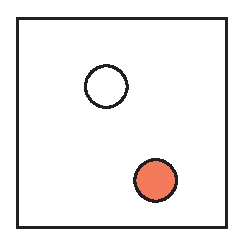
\includegraphics[width=1.5in]{sample.eps}
%  \caption{Lookit! Lookit!}
%}

%% Abstract section.
\abstract{TODO} % end of abstract

%% ACM Computing Classification System (CCS). 
%% See <http://www.acm.org/about/class> for details.
%% We recommend the 2012 system <http://www.acm.org/about/class/class/2012>
%% For the 2012 system use the ``\CCScatTwelve'' which command takes four arguments.
%% The 1998 system <http://www.acm.org/about/class/class/2012> is still possible
%% For the 1998 system use the ``\CCScat'' which command takes four arguments.
%% In both cases the last two arguments (1998) or last three (2012) can be empty.

\CCScatlist{
  \CCScatTwelve{Human-centered computing}{Visu\-al\-iza\-tion}{Visu\-al\-iza\-tion techniques}{Treemaps};
  \CCScatTwelve{Human-centered computing}{Visu\-al\-iza\-tion}{Visualization design and evaluation methods}{}
}

%\CCScatlist{
  %\CCScat{H.5.2}{User Interfaces}{User Interfaces}{Graphical user interfaces (GUI)}{};
  %\CCScat{H.5.m}{Information Interfaces and Presentation}{Miscellaneous}{}{}
%}

%% Copyright space is enabled by default as required by guidelines.
%% It is disabled by the 'review' option or via the following command:
% \nocopyrightspace

%%%%%%%%%%%%%%%%%%%%%%%%%%%%%%%%%%%%%%%%%%%%%%%%%%%%%%%%%%%%%%%%
%%%%%%%%%%%%%%%%%%%%%% START OF THE PAPER %%%%%%%%%%%%%%%%%%%%%%
%%%%%%%%%%%%%%%%%%%%%%%%%%%%%%%%%%%%%%%%%%%%%%%%%%%%%%%%%%%%%%%%%

\begin{document}

%% The ``\maketitle'' command must be the first command after the
%% ``\begin{document}'' command. It prepares and prints the title block.

%% the only exception to this rule is the \firstsection command
\firstsection{Introduction}

\maketitle

%% \section{Introduction} %for journal use above \firstsection{..} instead
TODO

\section{Related Work}

TODO

\section{Overview}

TODO
\begin{itemize}
  \item We visualize ligand trajectories
  \item We visualize energetic profiles
\end{itemize}

\begin{figure}[htb]
  \centering
  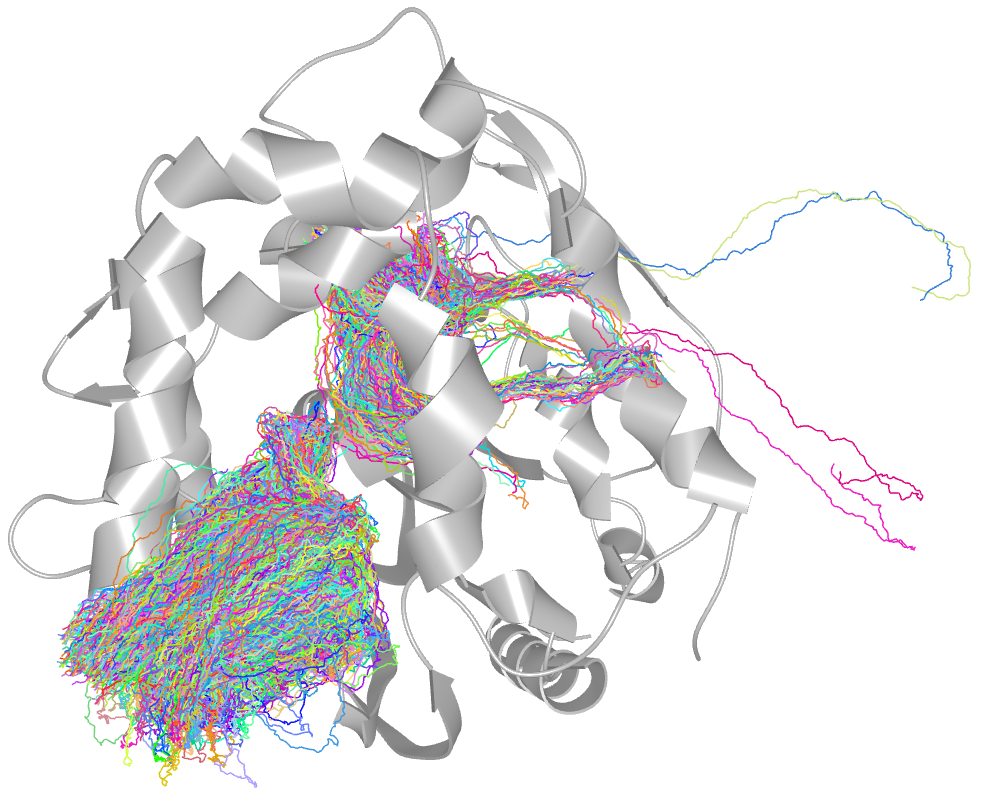
\includegraphics[width=\columnwidth]{trajectories}
  \caption{TODO replace, caption}
  \label{fig:trajectories}
\end{figure}

From the chemistry point of view, the binding energy of a ligand-substrate complex is an essential measure when evaluating the complex.
Therefore, we decided to strongly focus on conveying the binding energy when visualizing the trajectories dataset.
Naturally, this can be achieved by sampling the binding energy along a ligand trajectory and plotting the obtained data to a 2D chart.
In this manner, we obtain an abstraction of the trajectory in terms of the ligand binding energy profile (see Figure~\ref{fig:trajectory}).
Further, the energy profiles of the trajectories can be visualized within one 2D plot using superimposition.

\begin{figure}[htb]
  \centering
  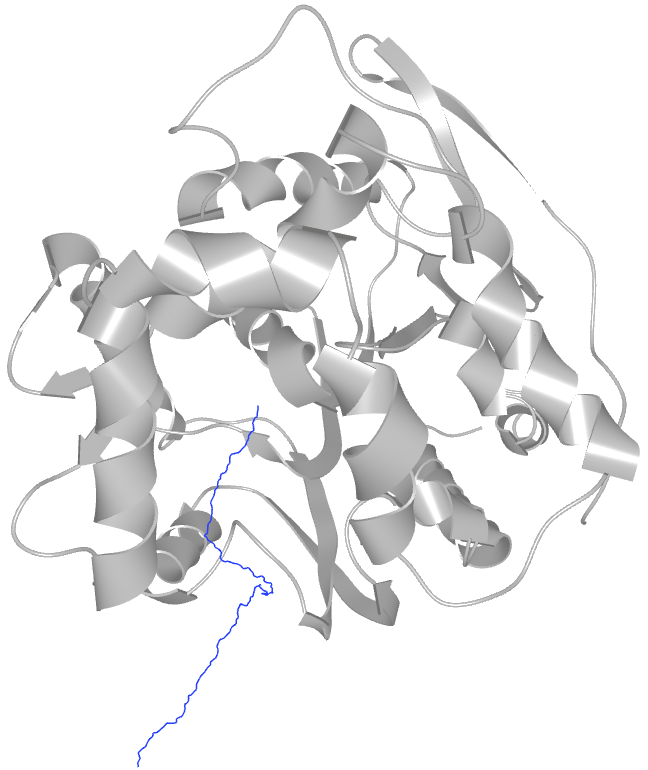
\includegraphics[width=0.5\columnwidth]{trajectory}\\
  \vspace{1em}
  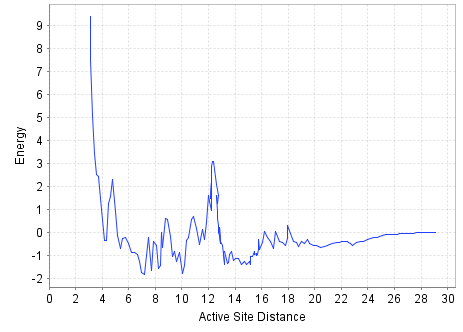
\includegraphics[width=0.8\columnwidth]{trajectory-energy}
  \caption{TODO figure quality, caption}
  \label{fig:trajectory}
\end{figure}

However, the superimposed visualization of energetic profiles does not scale well and becomes uninformative when visualizing hundreds (and more) trajectories (see Figure ?).
Particularly, there arise two issues for the users of such visualization. First, the main energetic trends become overshadowed, and second it is not possible to navigate to individual trajectories.
In order to overcome these issues, we propose a visualization system which employs well established visualization concepts in an interactive manner such that a ligand trajectories dataset can be explored based on the user needs.
Namely, we reduce the amount of energetic profiles visualized in a chart by binning the data by neighborhood and presenting it using small multiples approach.
Regarding the binning, we aim for as general as possible usage and therefore we let the user to control the data neighborhood measure.
We describe the approach in detail in Section 4.?.

\section{Visual Analysis of Trajectories}

TODO
\begin{itemize}
  \item figures of direct visualization of trajectories, profiles
\end{itemize}

\subsection{Small Multiples (Dataset Slicing)}

\paragraph{•} Properties -- In order to be able to slice the data, we first define an abstract representation of a ligand trajectory.
We decided to represent the trajectory using a set of 1D variables that we call trajectory properties.
Each trajectory property is defined such that it describes a specific characterstic of the trajectory.
We define the following properties:
\begin{itemize}
  \item \textbf{Minimum Distance to Active Site} --
  \item \textbf{Area Under Curve} --
  \item \textbf{?Energy Variance} --
  \item \textbf{Structure RMSD} --
  \item \textbf{Ligand Conformation Variance} --
\end{itemize}

\paragraph{•} Trends

\paragraph{•} Zooming

\subsection{3D Visualization}

\paragraph{•} Spatial Aggregation

\section{Evaluation}

TODO
\begin{itemize}
  \item LinBwt vs. LinB32 (W177 closes main tunnel)
\end{itemize}

\section{Discussion (+ Future Work)}

TODO
\begin{itemize}
  \item can be used also for CaverDock
\end{itemize}

\section{Conclusion}

%% if specified like this the section will be committed in review mode
\acknowledgments{TODO This work was supported in part by a grant from XYZ.}

%\bibliographystyle{abbrv}
\bibliographystyle{abbrv-doi}
%\bibliographystyle{abbrv-doi-narrow}
%\bibliographystyle{abbrv-doi-hyperref}
%\bibliographystyle{abbrv-doi-hyperref-narrow}

\bibliography{paper}
\end{document}
